\chapter{\ifenglish Conclusions and Discussions\else บทสรุปและข้อเสนอแนะ\fi}

\section{\ifenglish Conclusions\else สรุปผล\fi}

% นศ. ควรสรุปถึงข้อจำกัดของระบบในด้านต่างๆ ที่ระบบมีในเนื้อหาส่วนนี้ด้วย
จากผลการดำเนินงานนี้สามารถบรรลุวัตถุประสงค์ของโครงงานในการช่วยให้ผู้ใช้งานสามารถหาที่นั่งได้สะดวกมากยิ่งขึ้นและสามารถวางแผนล่วงหน้าได้ อีกทั้งผลประเมินความพึงพอใจโดยรวมเฉลี่ยถือว่าอยู่ในระดับที่ดี
แต่ยังมีข้อจำกัดในด้านของการแสดงผลที่ไม่ทั่วถึงเนื่องจากโครงงานนี้ทดสอบแค่ 3 โซนของบริเวณชั้น 2 ในสำนักหอสมุดมหาวิทยาลัยเชียงใหม่

\section{\ifenglish Challenges\else ปัญหาที่พบและแนวทางการแก้ไข\fi}

% ในการทำโครงงานนี้ พบว่าเกิดปัญหาหลักๆ ดังนี้
% \subsection{ในช่วงแรก ESP32-CAM with OV2640 ไม่สามารถส่งภาพไปยัง AWS S3 ได้}
% เนื่องจากยังไม่คุ้นชินกับการใช้ฟังก์ชันต่างๆ ของ AWS Web Service ทำให้ไม่สามารถส่งภาพจาก ESP32-CAM with OV2640 ได้ จึงแก้ไขให้ ESP32-CAM with OV2640 ส่งภาพไปเก็บไว้ที่ Google Drive ก่อนแล้วค่อย upload ไปยัง AWS S3 ทำให้การทำงานล่าช้าในช่วงแรกและซ้ำซ้อน 
% \subsection{ESP32-CAM with OV2640 ไม่สามารถเชื่อมต่อ WiFi ของ JumboPlus IoT ได้}
\begin{enumerate}
    \item ไม่สามารถ upload code ไปที่ ESP32-CAM with OV2640 ได้ ต้องทำการอัปเดต driver 
    \item ESP32-CAM with OV2640 ไม่สามารถเชื่อมต่อ WiFi ของ JumboPlus IoT ได้ จึงแก้ปัญหาโดยการแชร์ WiFi ของตนเองแทน
    \item ในช่วงแรก ESP32-CAM with OV2640 ไม่สามารถส่งภาพไปยัง AWS S3 ได้ เนื่องจากยังไม่คุ้นชินกับการใช้ฟังก์ชันต่างๆ ของ AWS Web Service 
    ทำให้ไม่สามารถส่งภาพจาก ESP32-CAM with OV2640 ได้ จึงแก้ไขให้ ESP32-CAM with OV2640 ส่งภาพไปเก็บไว้ที่ Google Drive ก่อนแล้วค่อย upload ไปยัง AWS S3 ทำให้การทำงานล่าช้าในช่วงแรกและซ้ำซ้อน
\end{enumerate}

\newpage
\section{\ifenglish%
Suggestions and further improvements
\else%
ข้อเสนอแนะและแนวทางการพัฒนาต่อ
\fi
}
% ข้อเสนอแนะเพื่อพัฒนาโครงงานนี้ต่อไป มีดังนี้
\subsection{ข้อเสนอแนะจากผู้ใช้งาน}
\begin{figure}[ht]
    \centering
    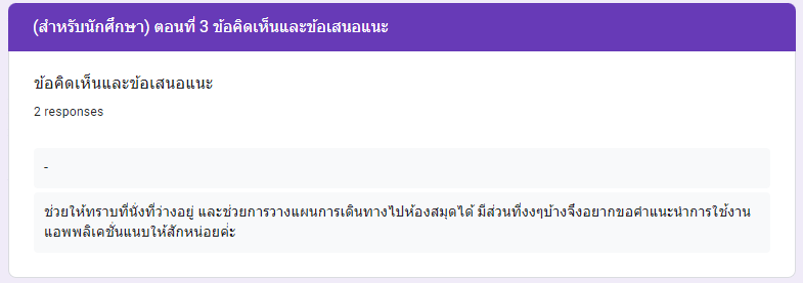
\includegraphics[scale=0.8]{images/student-s.png}
    \caption[st-s]{ข้อเสนอแนะจากนักศึกษา}
    \label{fig:st-s}
% \end{figure}
% \begin{figure}[ht]
    \centering
    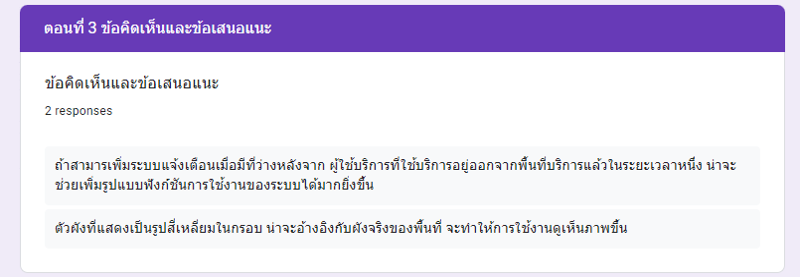
\includegraphics[scale=0.8]{images/cmul-s.png}
    \caption[cmul-s]{ข้อเสนอแนะจากทางสำนักหอสมุด}
    \label{fig:cmul-s}
\end{figure}

\subsection{ข้อเสนอแนะในการพัฒนาต่อ}
\subsection{ค่าใช้จ่ายในการพัฒนาต่อ}
